\documentclass[landscape]{article}
\usepackage{multicol}
\usepackage[margin=1in]{geometry}
\usepackage{clrscode3e}
\usepackage{amsmath}
\usepackage{graphicx}

\newcommand{\bi}{\begin{itemize}}
\newcommand{\ii}{\item}
\newcommand{\ei}{\end{itemize}}
\newcommand{\bn}{\begin{enumerate}}
\newcommand{\en}{\end{enumerate}}
\newcommand{\set}[1]{\ensuremath{\left\{#1\right\}}}
\newcommand{\pr}[1]{\ensuremath{\mbox{Pr}\left\{#1\right\}}}
\newcommand{\flr}[1]{\ensuremath{\left\lfloor#1\right\rfloor}}
\newcommand{\ceil}[1]{\ensuremath{\left\lceil#1\right\rceil}}

\newcommand{\sect}[1]{\newpage{\textbf{#1}}}

\setlength{\parindent}{0in}

\newcommand{\nop}[1]{}

\title{Notes on Linear Sorting}
\author{Geoffrey Matthews}
\begin{document}
\maketitle
\titlepage
\huge


\sect{Comparison sorts}
\bi
\ii The only operation that may be used to gain
information about a sequence is comparisons between pairs of elements.
\ii All sorts seen so far are comparison sorts:
\bi
\ii insertion sort
\ii merge sort
\ii quicksort
\ii heapsort
\ei
\ei

\sect{Lower bounds for comparison sorts}
\bi
\ii $\Omega(n)$ to examine all the input
\ii All sorts seen so far are $\Omega(n\lg n)$
\ii We will show that all comparison sorts must be $\Omega(n\lg n)$
\ei

\sect{Decision tree}
\bi
\ii Abstraction of any comparison sort
\ii Represents comparisons made by
\bi
\ii a specific sorting algorithm
\ii on inputs of a given size
\ei
\ii Abstracts away everything else: control and data movement.
\ii We're counting {\em only} comparisons.
\ei

\sect{Insertion sort on three elements}
\vspace{1cm}

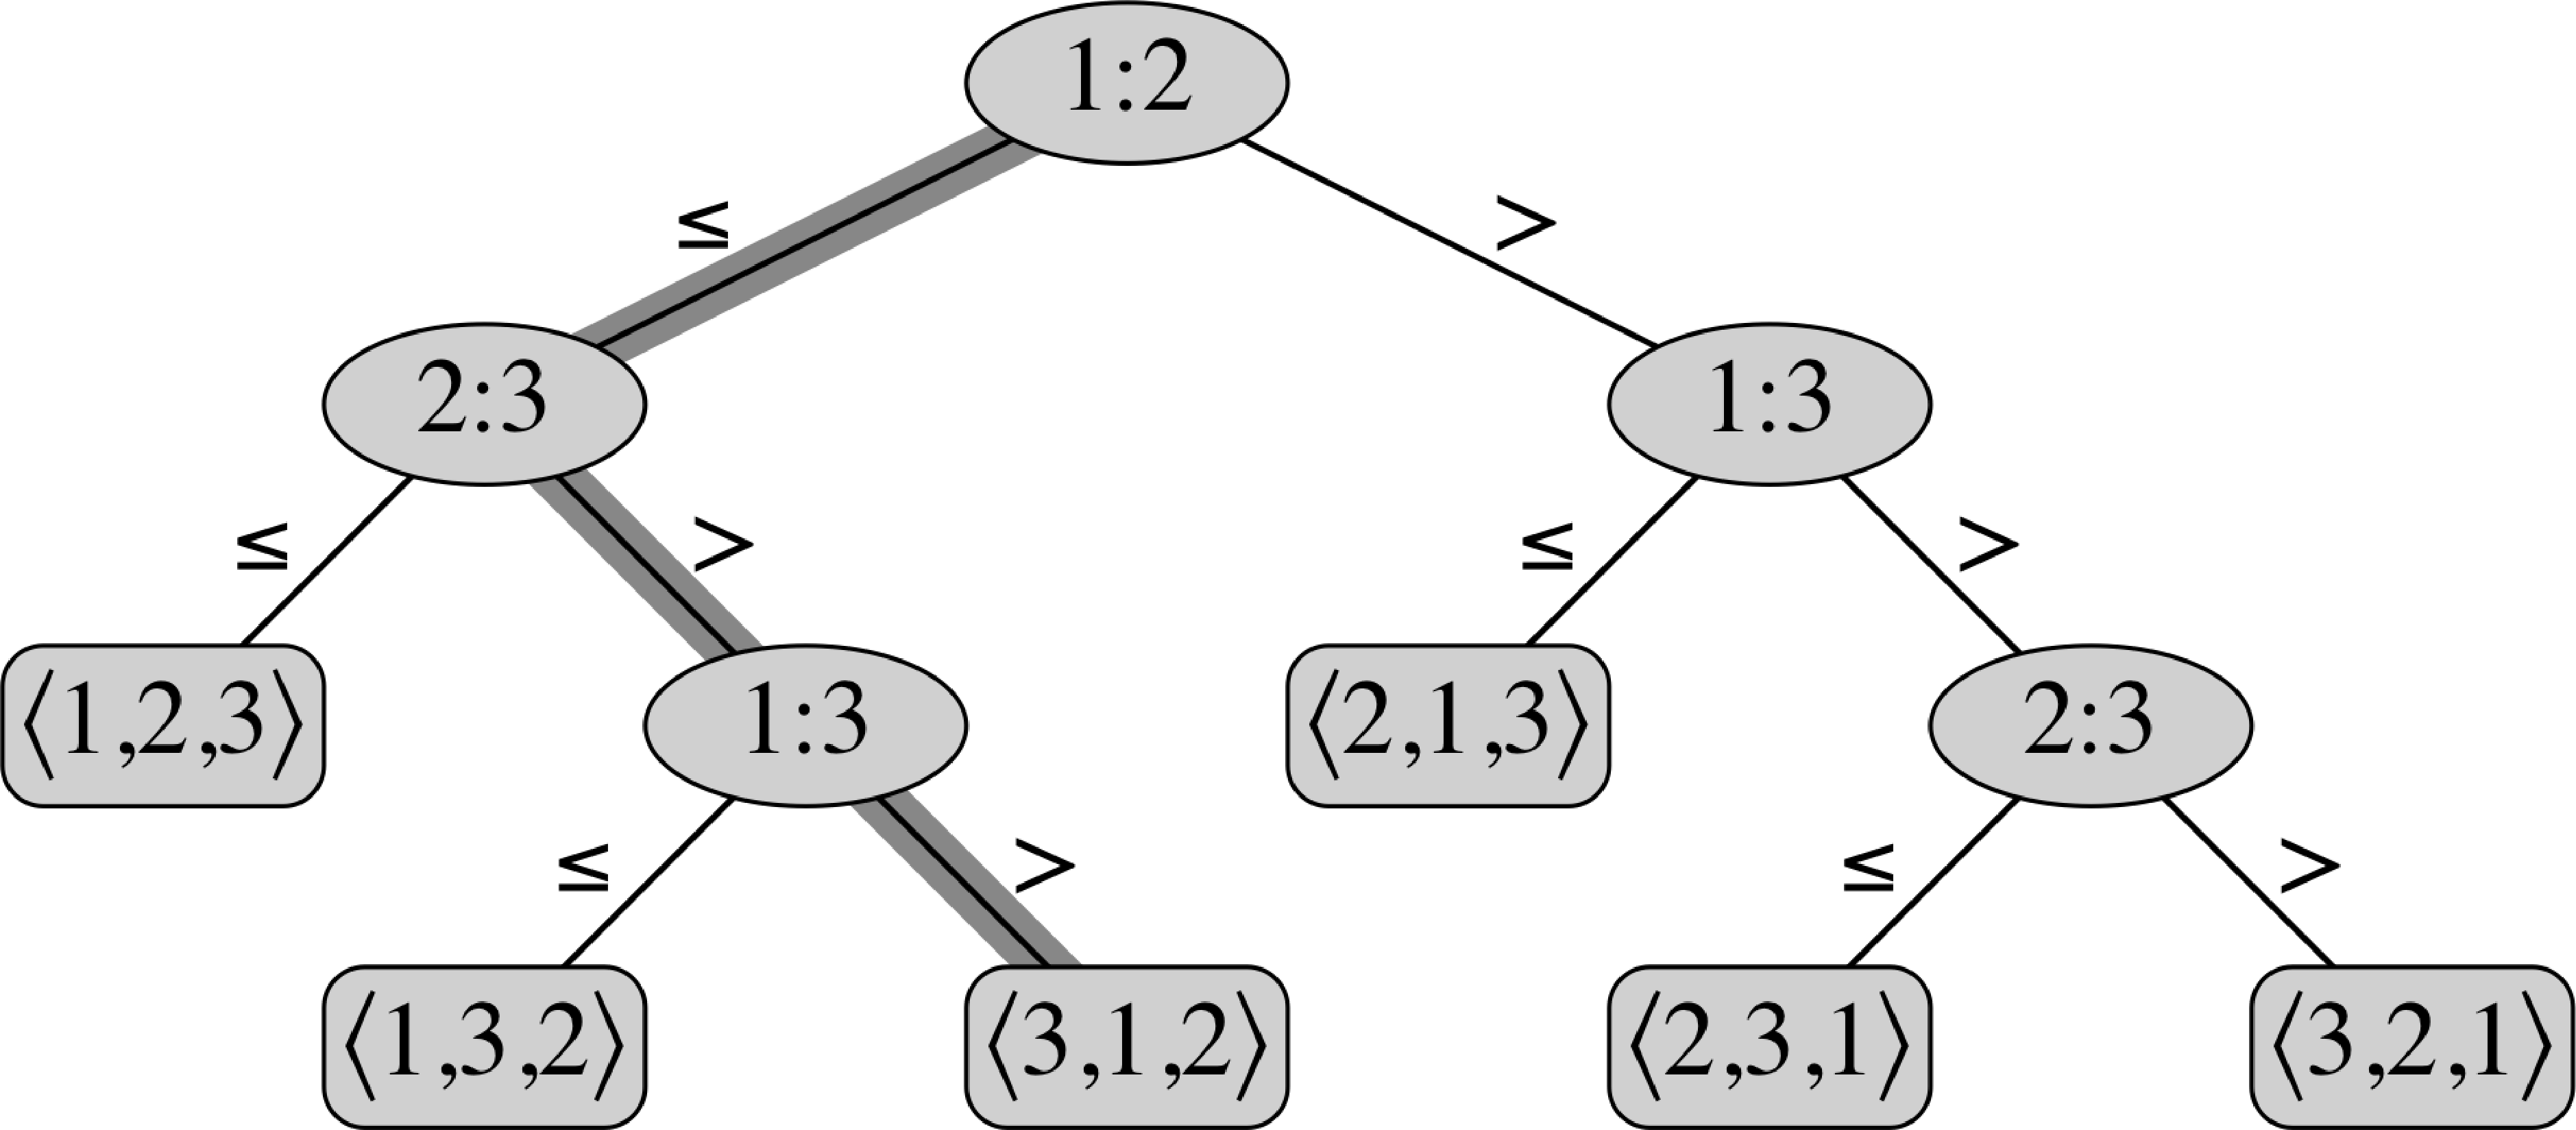
\includegraphics[width=\textwidth]{Fig-8-1.pdf}

\bi
\ii Internal nodes labeled by comparisons (original positions).
\ii Leaf nodes labeled by permutation of order from original.
\ii Number of leaves $\geq n!$.
\ei


\sect{For any comparison sort}

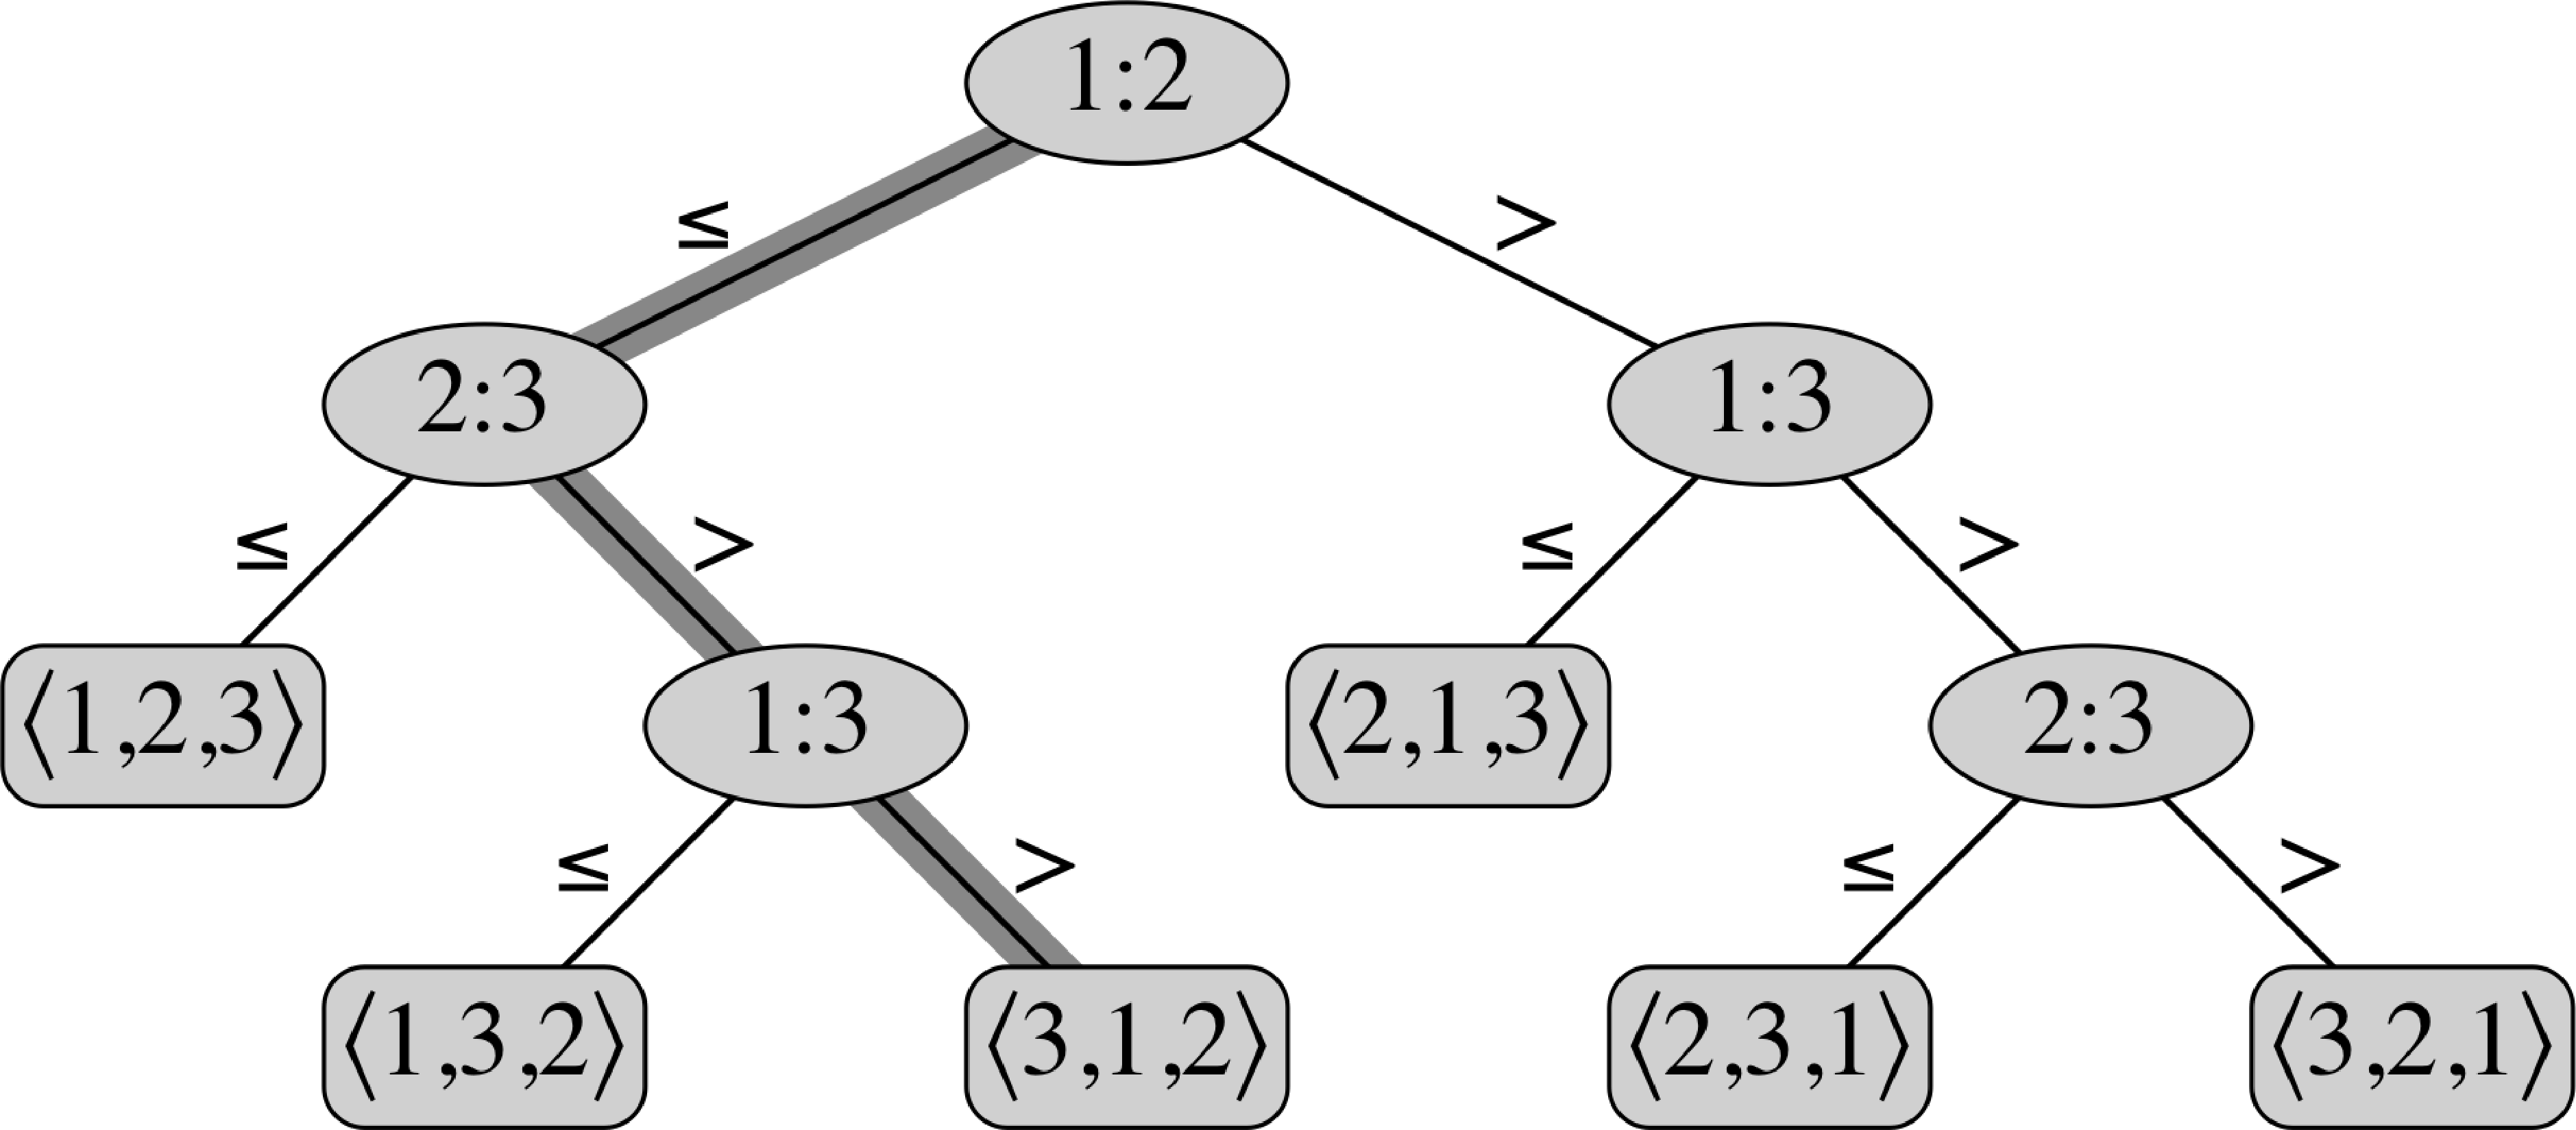
\includegraphics[width=\textwidth]{Fig-8-1.pdf}
\bi
\ii 1 tree for each $n$
\ii View the tree as if the algorithm splits in two at each node.
\ii The tree models all possible execution traces.
\ei

\sect{What is the longest path from root to leaf?}
\bi
\ii Depends on the algorithm.
\ii Insertion sort: $\Theta(n^2)$
\ii Merge sort: $\Theta(n\lg n)$
\ei

\sect{Lemma: any binary tree of height $h$ has $\leq 2^h$ leaves.}
\bi
\ii $\ell = $\# of leaves
\ii $h = $ height
\ii then $\ell \leq 2^h$
\ei
Proof by induction on $h$:
\begin{description}
  \item[Base:] $h=0$.  Tree is just one node, which is a
    leaf. $1 \leq 2^h$.
  \item[Inductive step:]
    Assume true for $h-1$.  Extend tree with as many new leaves as
    possible. Each leaf becomes the parent of two new leaves.
    \begin{align*}
      \mbox{\# of leaves for $h$} &= 2(\mbox{\# of leaves for $h-1$})\\
        &\leq 2(2^{h-1})\\
        &= 2^h
    \end{align*}
\end{description}


\sect{Theorem: any decision tree that sorts $n$ elements has height
  $\Omega(n\lg n)$ }
\bi
\ii $\ell \geq n!$
\ii $n! \leq \ell \leq 2^h$
\ii $h \geq \lg(n!)$
\ii Sterling's approximation: $n! > (n/e)^n$
\ii Therefore:
\begin{align*}
  h  &\geq \lg(n!)\\
  &\geq \lg(n/e)^n\\
  &= n\lg(n/e)\\
  &= n\lg n - n\lg e\\
  &= \Omega(n\lg n)
\end{align*}
\ei

\sect{Sorting in linear time}
\bi
\ii Impossible with any comparison sort.
\ii {\bf Counting sort}
\bi
\ii Key assumption:  numbers to be sorted are integers in $\{0,\ldots,k\}$.
\ei
\ei
\begin{description}
  \ii[Input:] $A[1..n]$ where $A[j] \in\{0,...,k\}$
  \ii[Output:] $B[1..n]$, sorted.
  \ii[Auxiliary storage:] $C[0..k]$
\end{description}



\sect{Counting sort example}
\begin{multicols}{2}
\begin{codebox}
  \Procname{$\proc{Counting-Sort}(A,B,n,k)$}
  \li let $C[0..k]$ be a new array
  \li \For $i\gets 0$ \To $k$ \Do
  \li $C[i] \gets 0$ \End
  \li \For $j\gets 1$ \To $n$ \Do
  \li $C[A[j]] \gets C[A[j]]+1$ \End
  \li \For $i\gets 1$ \To $k$ \Do
  \li $C[i] \gets C[i] + C[i-1]$ \End
  \li \For $j \gets n$ \Downto $1$ \Do
  \li $B[C[A[j]]] \gets A[j]$
  \li $C[A[j]] \gets C[A[j]]-1$ \End
\End
\end{codebox}
\columnbreak



{\bf A:}\begin{tabular}{|c|c|c|c|c|c|c|c|}\hline
 $2_1$ & $5_1$ & $3_1$ & $0_1$ & $2_2$ & $3_2$ & $0_2$ & $3_3$ \\\hline
\end{tabular}\\

After second {\bf for} loop:\\
{\bf C:}\begin{tabular}{|c|c|c|c|c|c|c|c|}\hline
 2 & 0 & 2 & 3 & 0 & 1\\\hline
  \end{tabular}\\


After third {\bf for} loop:\\
{\bf C:}\begin{tabular}{|c|c|c|c|c|c|c|c|}\hline
 2 & 2 & 4 & 7 & 7 & 8\\\hline
  \end{tabular}


\end{multicols}
\sect{Counting sort example}
\begin{multicols}{2}
\begin{codebox}
  \Procname{$\proc{Counting-Sort}(A,B,n,k)$}
  \li let $C[0..k]$ be a new array
  \li \For $i\gets 0$ \To $k$ \Do
  \li $C[i] \gets 0$ \End
  \li \For $j\gets 1$ \To $n$ \Do
  \li $C[A[j]] \gets C[A[j]]+1$ \End
  \li \For $i\gets 1$ \To $k$ \Do
  \li $C[i] \gets C[i] + C[i-1]$ \End
  \li \For $j \gets n$ \Downto $1$ \Do
  \li $B[C[A[j]]] \gets A[j]$
  \li $C[A[j]] \gets C[A[j]]-1$ \End
\End
\end{codebox}
\columnbreak


{\bf A:}
\begin{tabular}{|c|c|c|c|c|c|c|c|}\hline
 $2_1$ & $5_1$ & $3_1$ & $0_1$ & $2_2$ & $3_2$ & $0_2$ & $3_3$ \\\hline
\end{tabular}\\

{\bf C:}\begin{tabular}{|c|c|c|c|c|c|c|c|}\hline
 2 & 2 & 4 & 7 & 7 & 8\\\hline
  \end{tabular}\\

{\bf B:}
\begin{tabular}{|c|c|c|c|c|c|c|c|}\hline
 & & & & & & $3_3$ & \\\hline
 & $0_2$ & & & & & $3_3$ & \\\hline
 & $0_2$ & & & & $3_2$ & $3_3$ & \\\hline
 & $0_2$ & & $2_2$ & & $3_2$ & $3_3$ & \\\hline
$0_1$ & $0_2$ & & $2_2$ & & $3_2$ & $3_3$ & \\\hline
$0_1$ & $0_2$ & & $2_2$ & $3_1$ & $3_2$ & $3_3$ & \\\hline
$0_1$ & $0_2$ & & $2_2$ & $3_1$ & $3_2$ & $3_3$ & $5_1$\\\hline
$0_1$ & $0_2$ & $2_1$ & $2_2$ & $3_1$ & $3_2$ & $3_3$ & $5_1$\\\hline
\end{tabular}\\


\end{multicols}

 Counting sort is {\bf stable}:
\bi
\ii Keys with the same value appear in the same order
in output as in input.
\ei

\sect{Counting sort analysis}
\begin{multicols}{2}
\begin{codebox}
  \Procname{$\proc{Counting-Sort}(A,B,n,k)$}
  \li let $C[0..k]$ be a new array
  \li \For $i\gets 0$ \To $k$ \Do
  \li $C[i] \gets 0$ \End
  \li \For $j\gets 1$ \To $n$ \Do
  \li $C[A[j]] \gets C[A[j]]+1$ \End
  \li \For $i\gets 1$ \To $k$ \Do
  \li $C[i] \gets C[i] + C[i-1]$ \End
  \li \For $j \gets n$ \Downto $1$ \Do
  \li $B[C[A[j]]] \gets A[j]$
  \li $C[A[j]] \gets C[A[j]]-1$ \End
\End
\end{codebox}
\columnbreak

\bi
\ii $\Theta(n+k)$
\bi\ii which is $\Theta(n)$ if $k=O(n)$.\ei
\ii How big a $k$ is practical?
\bi
\ii 32-bit values?  No.
\ii 16-bit?  Probably not.
\ii 8-bit?  Maybe, depending on $n$.
\ii 4-bit? Unless $n$ is really small.
\ei
\ei
\end{multicols}
\vfill

\bi
\ii Counting sort will be used in radix sort.
\ei
\vfill


\sect{Radix sort example}

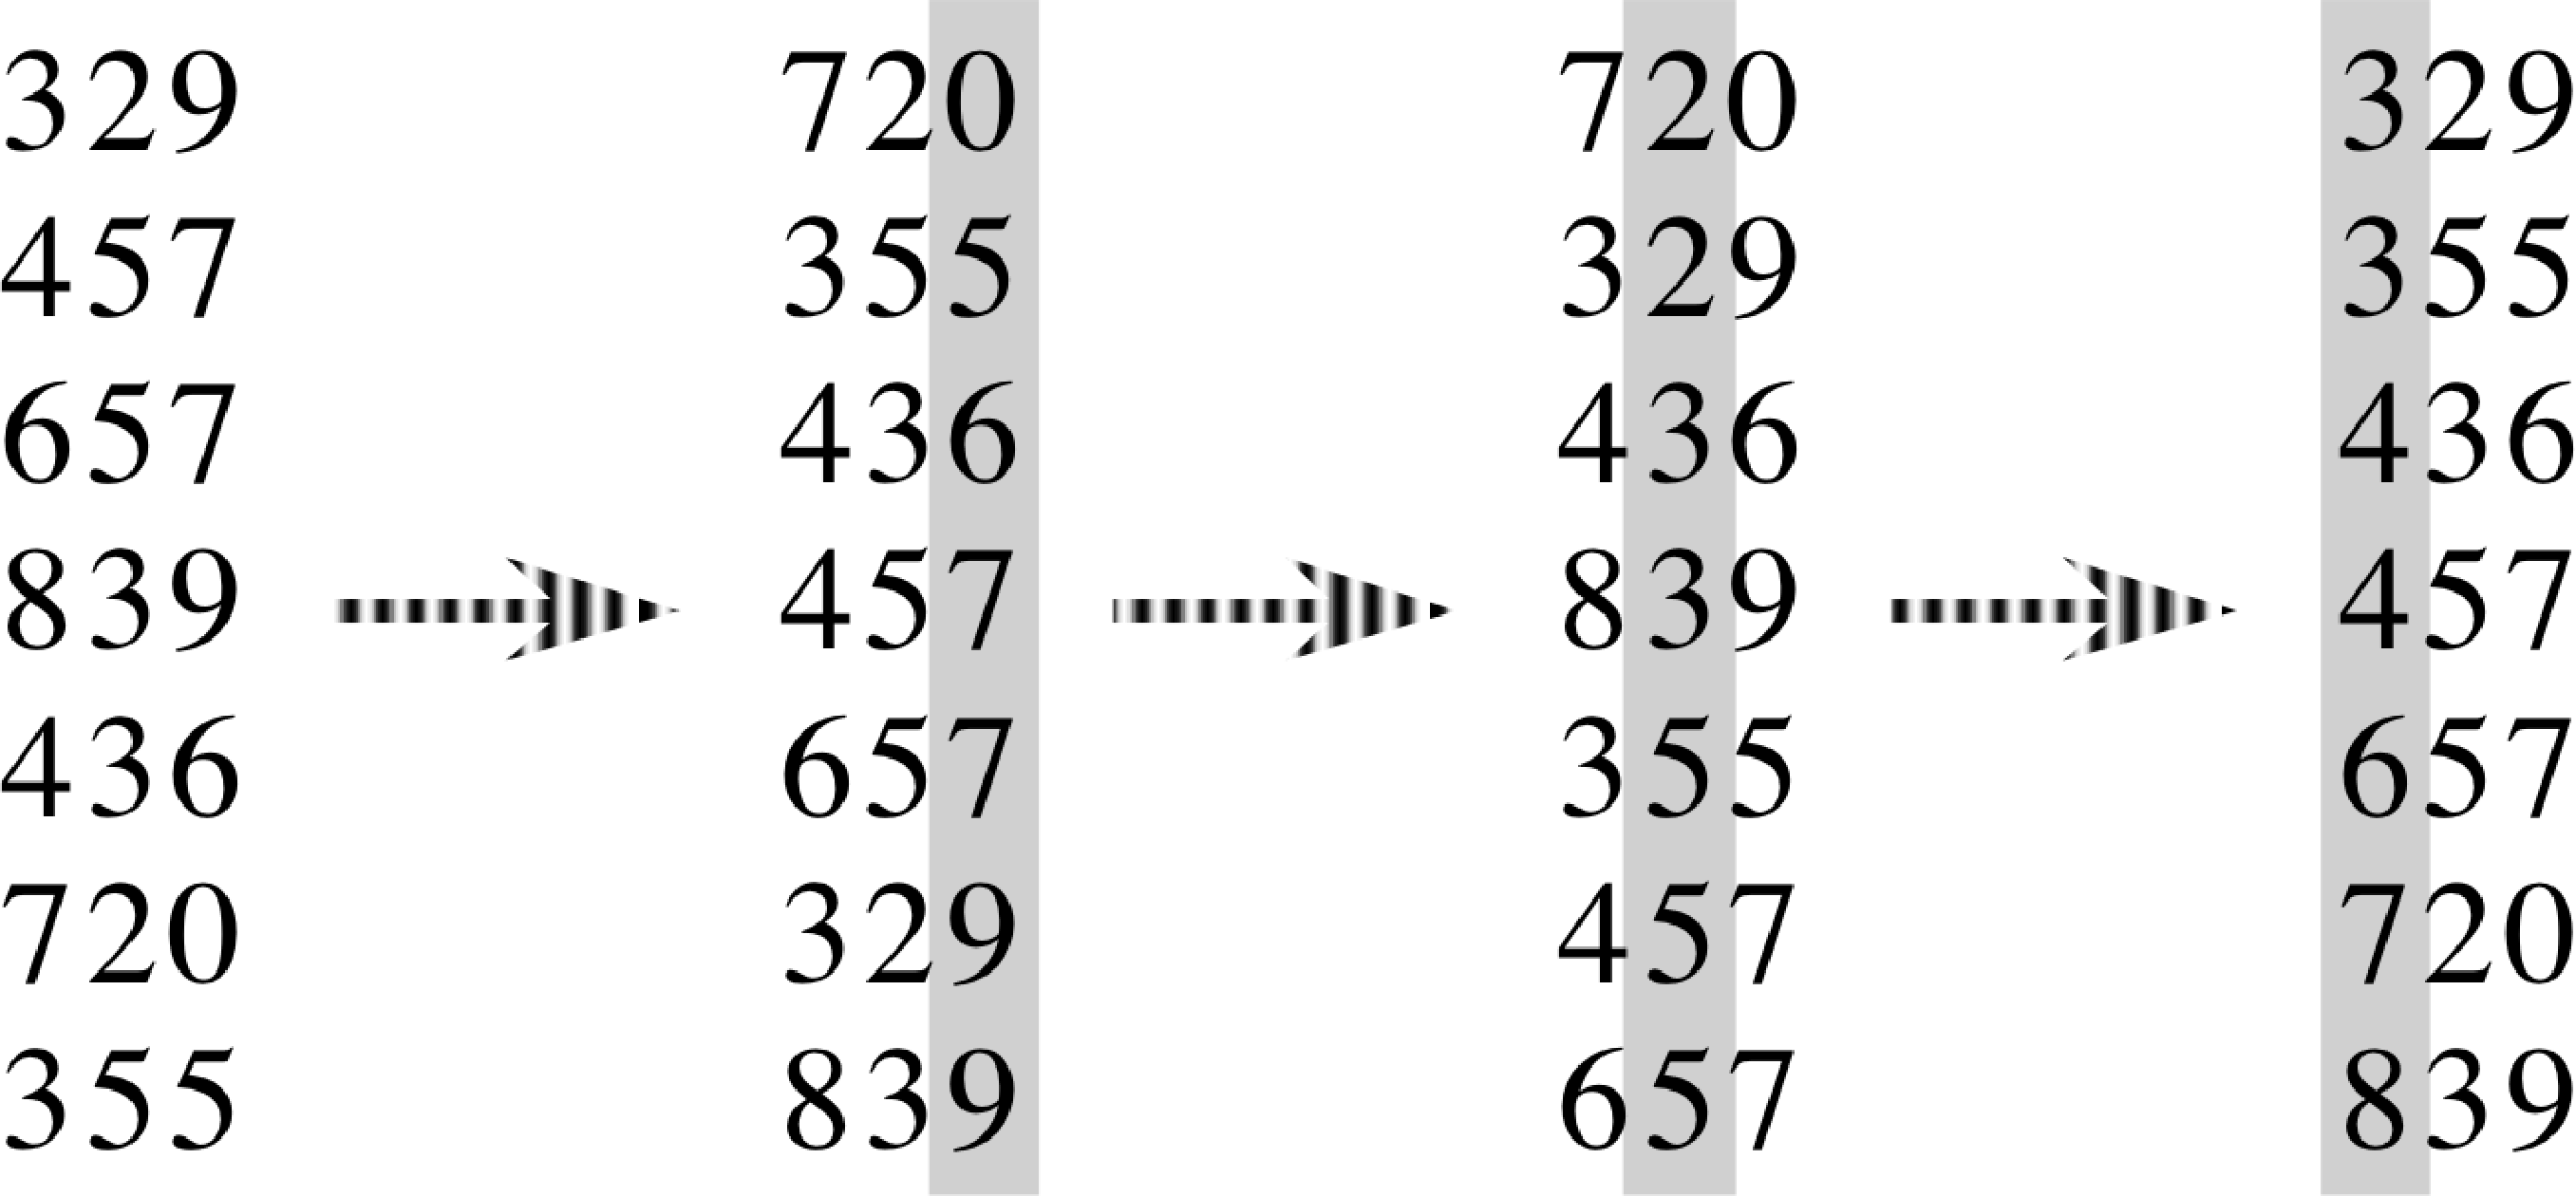
\includegraphics[width=\textwidth]{Fig-8-3.pdf}

\sect{Radix sort}

\vfill

\begin{minipage}[b]{0.45\textwidth}
\bi
\ii IBM in early 20th century.
\ii Punch card sorting machines only sorted on one column.
\ii Humans would reload the cards and change the column.
\ii Human-machine cyborg algorithm!
\ei
\begin{description}
  \ii[Key idea:]\mbox{}\\ Sort {\em least} significant digits first.
\end{description}
\end{minipage}\hfill
\begin{minipage}{0.5\textwidth}
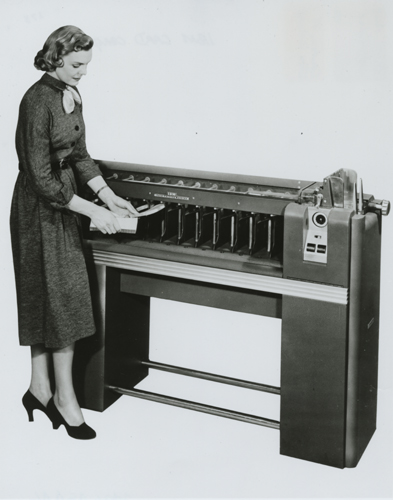
\includegraphics[width=\textwidth]{ibmcardsorter.jpg}
\end{minipage}

\sect{Radix sort}
\begin{codebox}
  \Procname{$\proc{Radix-Sort}(A,d)$}
  \li \For $i\gets 1$ \To $d$ \Do
  \li use a stable sort to sort $A$ on digit $i$
  \End
\end{codebox}

\sect{Radix sort correctness}
\bi
\ii Induction on number of passes.
\ii Assume digits $1,\ldots,i-1$ are sorted.
\ii Show that a stable sort on $i$ leaves $1,\ldots,i-1$ sorted:
\bi
\ii If 2 digits in position $i$ are different,
\bi \ii ordering by $i$ is
correct and positions $1,\ldots,i-1$ are irrelevant.
\ei
\ii If 2 digits in position $i$ are equal,
\bi \ii numbers are already sorted
by inductive hypothesis.  Stable sort leaves them that way.
\ei
\ei
\ei

\sect{Radix sort analysis}

Assume we use counting sort on each digit.
\bi
\ii $\Theta(n+k)$ per digit
\ii $d$ digits
\ii $\Theta(d(n+k))$ total
\ii If $k=O(n)$, time $= \Theta(dn)$.
\ei

\sect{Radix sort: How to break each key into digits?}
\bi
\ii $n$ words
\ii $b$ bits/word
\ii Break into $r$-bit digits.  $d=\lceil b/r \rceil$
\ii Use counting sort, $k = 2^r-1$.

Example: 32-bit words, 8-bit digits.
\begin{align*}
  b &= 32 & r &= 8 \\
  d &= \lceil 32/8\rceil = 4 & k &= 2^8-1 = 255
\end{align*}

\ii Time $=\Theta\left(\frac{b}{r}(n+2^r)\right)$
\ei

\sect{How to choose $r$?}
\bi

\ii Time $=\Theta\left(\frac{b}{r}(n+2^r)\right)$
\ii Balance $b/r$ and $n+2^r$.
\ii Choosing $r \approx \lg n$ gives
\[
\Theta\left(\frac{b}{\lg n}(n+n)\right) = \Theta(bn/\lg n)
\]
\ii If we choose $r < \lg n$ then $b/r > b/\lg n$ and $n+2^r$ doesn't
improve.
\ii If we choose $r > \lg n$ then $n+2^r$ term gets big.
\ii Sort $2^{16}$ 32-bit numbers, use $r=\lg 2^{16} = 16$
bits. $\lceil b/r \rceil = 2$ passes.
\ei

\sect{Compare radix to merge and quick}
\bi
\ii 1 million ($2^{20}$) 32-bit integers.
\ii Radix sort: $\lceil 32/20 \rceil = 2$ passes.
\ii Merge/quick: $\lg n = 20$ passes.
\ii Each radix ``pass'' is 2 passes:
\bi \ii one to take census
\ii one to move data \ei
\ei

\sect{How does radix sort violate the $\Omega(n\lg n)$ speed limit?}
\bi
\ii Counting sort allows us to gain information
about keys\bi\ii other than by directly comparing 2 keys.\ei
\ii Used keys as array indices,
\bi\ii thus getting far more information out
of each key.
\ii branching factor of the decision tree is $k$
\ei
\ei

\end{document}
